\documentclass[10pt,twocolumn,letterpaper]{article}

\usepackage{cvpr}
\usepackage{times}
\usepackage{epsfig}
\usepackage{graphicx}
\usepackage{amsmath}
\usepackage{amssymb}

% Include other packages here, before hyperref.

% If you comment hyperref and then uncomment it, you should delete
% egpaper.aux before re-running latex.  (Or just hit 'q' on the first latex
% run, let it finish, and you should be clear).
\usepackage[breaklinks=true,bookmarks=false]{hyperref}

\cvprfinalcopy % *** Uncomment this line for the final submission

\def\cvprPaperID{****} % *** Enter the CVPR Paper ID here
\def\httilde{\mbox{\tt\raisebox{-.5ex}{\symbol{126}}}}

% Pages are numbered in submission mode, and unnumbered in camera-ready
%\ifcvprfinal\pagestyle{empty}\fi
\setcounter{page}{1}
\begin{document}

%%%%%%%%% TITLE
\title{Neural Image Style Transfer}

\author{Veronica Lee\\
Massachusetts Institute of Technology\\
Cambridge, MA, USA\\
{\tt\small vslee@mit.edu}
% For a paper whose authors are all at the same institution,
% omit the following lines up until the closing ``}''.
% Additional authors and addresses can be added with ``\and'',
% just like the second author.
% To save space, use either the email address or home page, not both
\and
Samuel Song\\
Massachusetts Institute of Technology\\
Cambridge, MA, USA\\
{\tt\small samjsong@mit.edu}
}

\maketitle
%\thispagestyle{empty}

%%%%%%%%% ABSTRACT
\begin{abstract}
A pastiche is a work of art that imitates the style of other works of art. The computer vision and machine learning technologies that exist today allow pastiches to be created digitally. This automated process of recomposing an image to consist of styles from other images is called an image style transfer. In this paper, we discuss the reimplementation of image style transfer using a deep convolutional neural network, following the process outlined by Leon A. Gatys, Alexander S. Ecker, and Matthias Bethge [1]. We also discuss color mapping techniques which preserve the color of the content image.
\end{abstract}

%%%%%%%%% BODY TEXT
\section{Introduction}

A pastiche is a work of art that imitates the style of other works of art. The computer vision and machine learning technologies that exist today allow pastiches to be created digitally. Specifically, this automated process of recomposing an image (content image) to consist of styles from other images (style images) is called an image style transfer. 

Image style transfers are currently being used on mobile and web applications. These interfaces allow users to render any photograph with the style of a painting of their choice.

In this paper, we will discuss the implementation of image style transfer using a deep neural network, following the process outlined by Leon A. Gatys, Alexander S. Ecker, and Matthias Bethge [1]. In particular, we will use a convolutional neural network (CNN), which is a type of deep neural network favored for image processing tasks. 

The algorithm for neural image transfer produces an image that takes its color from the style image. We will also discuss color mapping techniques which preserve the color of the content image.

%------------------------------------------------------------------------
\section{Related Work}

While we are reimplementing the algorithm for neural image transfer in this paper, there have been many other works regarding image style transfer. 

Using neural networks to perform an image style transfer as in [1] is very recent breakthrough. Computing using neural networks, however, are computationally expensive. Optimizations have been performed [3, 4] to speed up the process. One improvement has been to frame the transfer from the style image to the content image as an image transformation problem and solve it by training a feed-forward, convolutional neural network. 

Following these time optimizations, there has recently been an implementation for video style transfer, which transfers the style of a painting to an entire video sequence, by Manuel Ruder et al [5]. In order to extend image style transfer to videos, they used new initializations and loss functions that improved frame-to-frame stability. 

There are approaches to implementing image style transfers that do not use deep convolutional neural networks. One example is the patch-based style transfer, which transfers the style by applying a patch in the style image that matches a patch in the content image. A disadvantage of this approach, however, is that the algorithm fails to transfer edge styles. 

%Another example is texture synthesis. 

%------------------------------------------------------------------------
\section{Definitions}

Generating image contents and image styles is defined as follows [1]:

Convolutional neural networks consist of layers of image filters, and the output of each layer is a feature map. The feature maps of the lower levels in the network will consist of exact pixel values from the original content image, while features from the higher levels will contain higher-level content information. Thus, we define content representation to be the outputs of the higher layers in the network.

We can add a feature space that obtains texture information to the network. If this feature space is built on top of the outputs of each level in the network, then we can acquire a correlation between the filter responses and the spatial extent of the feature maps. Thus, we define style representation to be the outputs of multiple layers in the supplemented network. 

Then the single convolutional neural network can generate both content representation (from higher levels of the original network) and style representation (across all levels of the supplemented network). This algorithm for neural image transfer thus highlights the ability to separate image contents and image styles into content representation and style representation. 

\begin{figure*}
\begin{center}
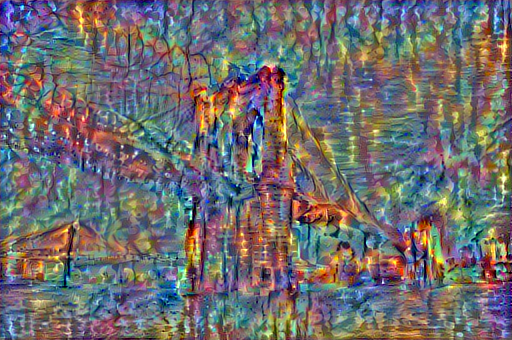
\includegraphics[width=0.3\linewidth]{painted_bridge/out_100.png}
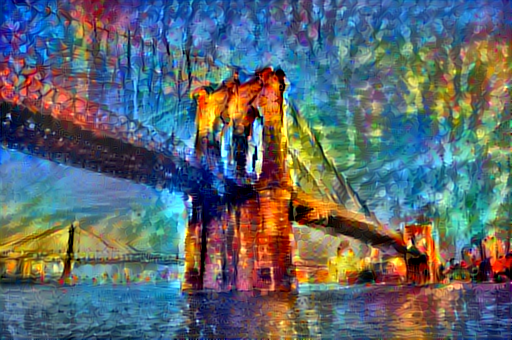
\includegraphics[width=0.3\linewidth]{painted_bridge/out_500.png}
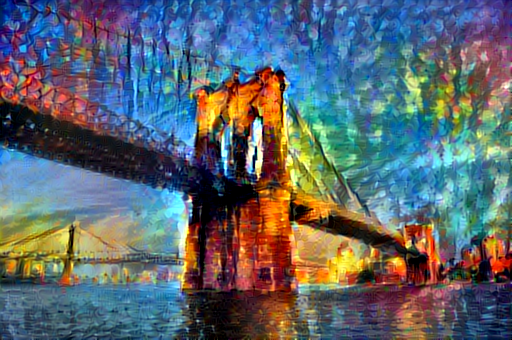
\includegraphics[width=0.3\linewidth]{painted_bridge/out.png}
\end{center}
   \caption{The generated images after 100, 500, and 1000 iterations. Does not preserve the color of the original image.}
\label{fig:short}
\end{figure*}

\begin{figure*}
\begin{center}
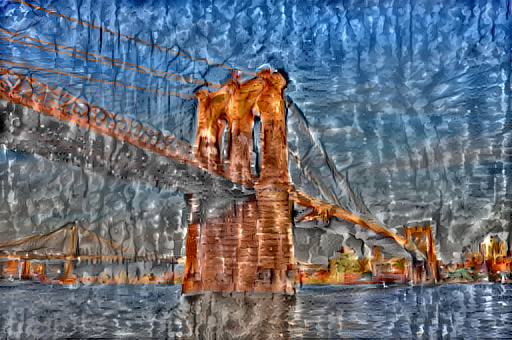
\includegraphics[width=0.3\linewidth]{painted_bridge_oc/out_100.png}
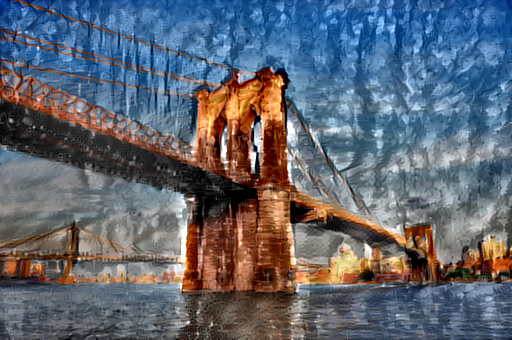
\includegraphics[width=0.3\linewidth]{painted_bridge_oc/out_500.png}
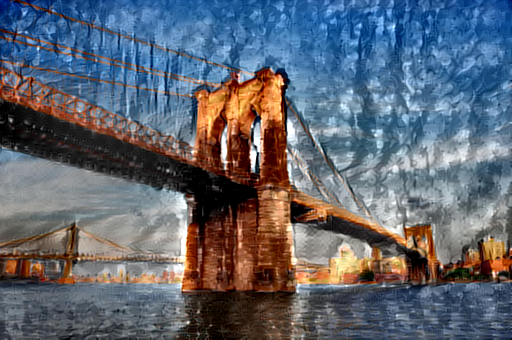
\includegraphics[width=0.3\linewidth]{painted_bridge_oc/out.png}
\end{center}
   \caption{The generated images after 100, 500, and 1000 iterations. Preserves the color of the original image.}
\label{fig:short}
\end{figure*}

%------------------------------------------------------------------------
\section{Image Style Transfer Using Neural Networks}

We followed the same methodology as outlined in [1]. In particular, we used the same 19-layer VGG network with 16 convolutional layers and 5 pooling layers, as given in [6], and normalized the VGG network by scaling weights. The model was publicly available in caffe [7]. We also used average pooling instead of maximum pooling, as suggested in [1].

Given that we were students enrolled in 6.819 and were allowed to reference other pre-trained models for guidance, we used [8] as a resource to guide us with the code implementation.

\subsection{Neural Algorithm}

The algorithm we implemented performs gradient descent on an initially white noise image to learn from our content and style images, synthesizing a new image, $\vec{x}$. We use the original 19-layer VGG net to generate this combined image. In each layer $l$ with $N_l$ distinct filters, we have $N_l$ feature maps of size $M_l$. Then we can represent our feature responses in each layer $l$ as

\[ F^l = \mathbb{R}^{N_l \times M_l} , \]
where $F_{ij}^l$ is the activation of the $i$th filter at position $j$ in layer $l$, as seen in [1].
\newline

\subsection{Content Representation}

To take the content of the photograph $\vec{p}$, we find the feature representations $P^l$ in layer $l$. Then the loss function we wish to minimize is

 \[ L_{\text{content}} ( \vec{p}, \vec{x}, l ) = \frac{1}{2} \sum_{i,j} (F_{ij}^l - P_{ij}^l)^2 \]
and the partial derivative with respect to activations is

\[ \frac{ \partial L}{\partial F_{ij}^l} = \left\{
    \begin{array}{ll}
          (F^l - P^l)_{ij} &\text{if} \ F_{ij}^l > 0 \\
         0 & \text{otherwise} \\
    \end{array} 
\right. \]

After each iteration of back propagation, our algorithm will make the proper changes to the output image $\vec{x}$ that minimize the loss with respect to the features of the content image.

\subsection{Style Representation}

To take the style of the artwork $\vec{a}$, we cannot use the features as is. In order to ignore the content and only consider the texture, we use the Gram matrix $G^l \in \mathbb{R}^{N_l \times N_l}$, where
\[ G_{ij}^l = \sum_k F_{ik}^l F_{jk}^l , \]
as seen in [1]. We do a similar process as above. We let $A^l$ be the Gram matrix that represents the style of the artwork $\vec{a}$, and define the loss function to be
\[ L_{\text{style}}(\vec{a}, \vec{x}) = \sum_{l = 0}^{K} w_l E_l \]
where
\[ E_l = \frac{1}{4N_l^2 M_l^2} \sum_{i,j} (G_{ij}^l - A_{ij}^l)^2 \]
is the error in each layer $l$, $w_l$ is the weight we give the layer $l$'s error, and $K$ is the total number of layers. We use the same weights $w_l$ as seen in [1].

The derivatives of $E_l$ are
\[ \frac{ \partial E_l}{\partial F_{ij}^l} = \left\{
    \begin{array}{ll}
         \frac{1}{N_l^2 M_l^2} ((F^l)^T (G^l - A^l))_{ji} &\text{if} \ F_{ij}^l > 0 \\
         0 & \text{otherwise} \\
    \end{array} 
\right. \]
This again allows us to run back propagation to make the proper changes to the output image $\vec{x}$ that minimize the loss.

\subsection{Style Transfer}

In order to combine the two processes we describe above, we define a third loss function
\[ L_{\text{total}}(\vec{p}, \vec{a}, \vec{x}) = \alpha L_{\text{content}}(\vec{p}, \vec{x}) + \beta L_{\text{style}} (\vec{a}, \vec{x}) \]
that is a linear combination of the two loss functions we defined above. At each iteration of our algorithm we generate the image that minimizes the combined error between the image and both the photograph (content) and artwork (style). 

\subsection{Color Mapping}

The algorithm for neural image transfer produces an image that takes its color from the style image, so we implemented color mapping to generate a final recomposed image that kept the colors of the content image but had the style from the style image. We considered the approaches given in [2] and decided to implement a simple version of the luminance-only transfer. In YUV image format, the Y channel contains luminance information and the UV channels hold color information. Thus, we implemented color mapping by post-processing the recomposed image [8], by taking the Y channel of the recomposed image, which had the colors of the style image, and the UV channels of the original content image to form a new recomposed image, which had the colors of the content image. 

%------------------------------------------------------------------------
\section{Results}

To test our implementation, we used the following photograph of the Brooklyn Bridge [9] as the content image,\begin{center}
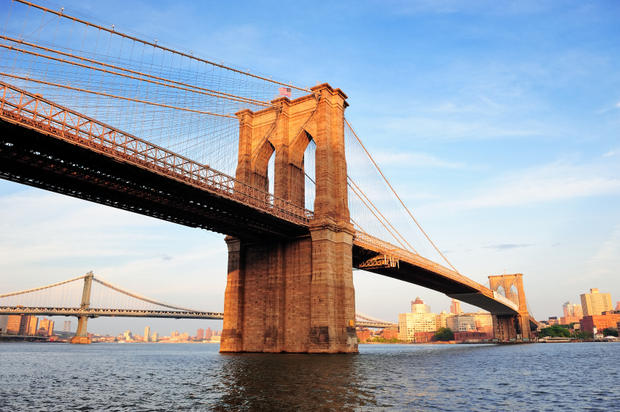
\includegraphics[width=0.8\linewidth]{content1.jpg}
\end{center}
and the following painting of a nighttime scene [10] as the style image.
\begin{center}
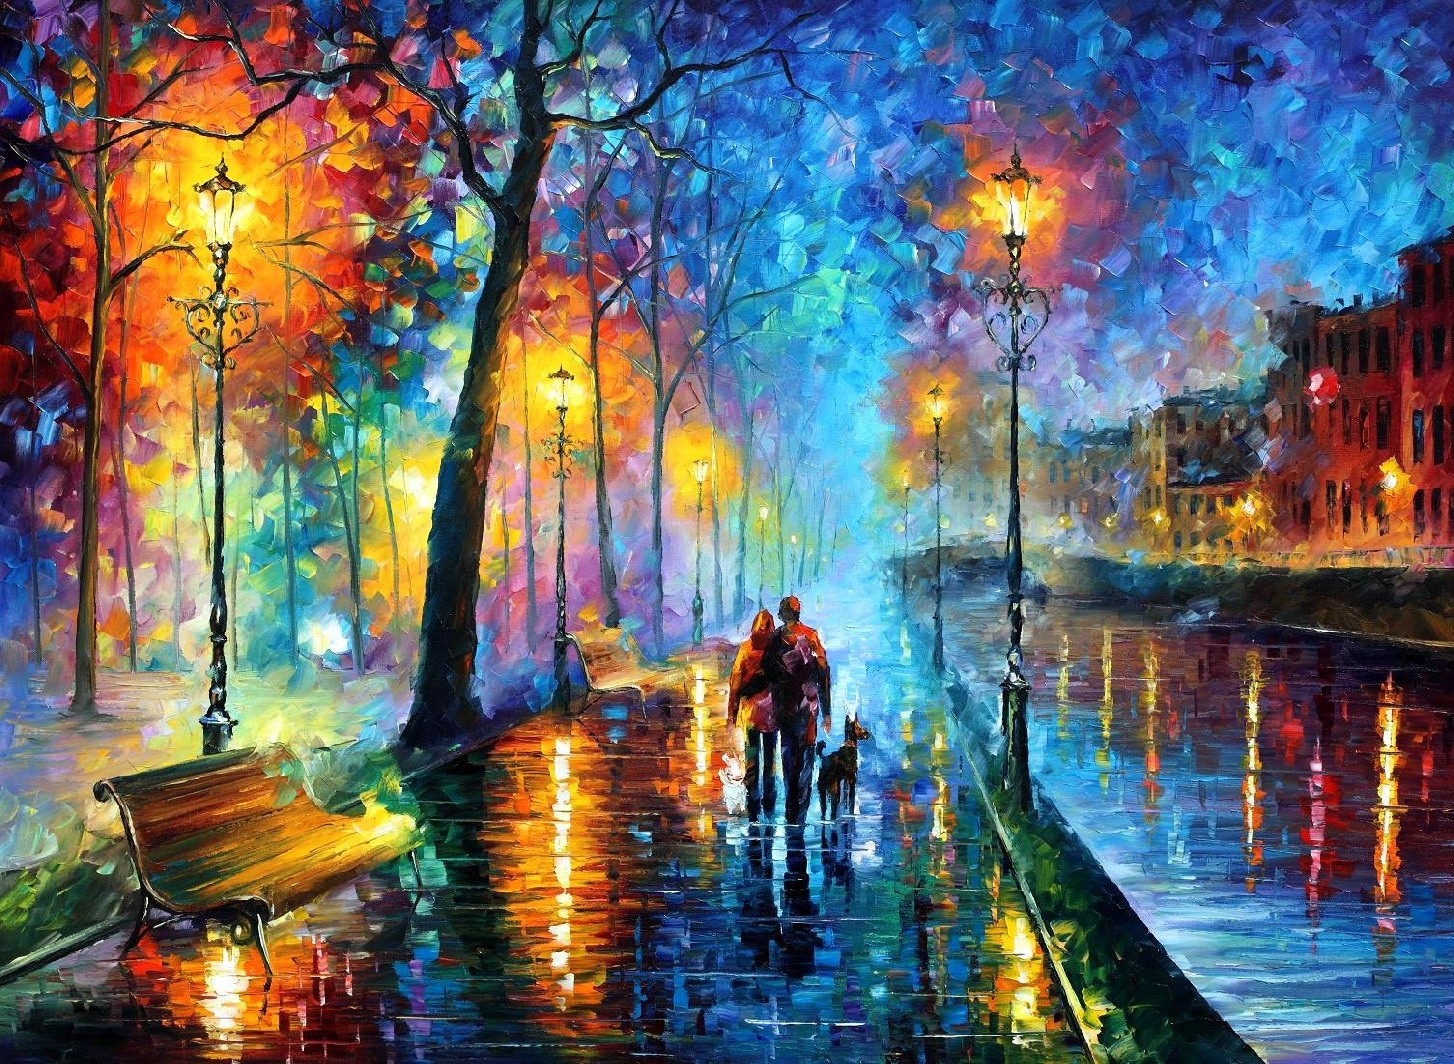
\includegraphics[width=0.8\linewidth]{style1.jpeg}
\end{center}

After trying different $\alpha$ and $\beta$ values, we chose to set $\alpha = 5$ and $\beta = 100$, as in [8], as those parameters gave us aesthetically pleasing results. 

Figure 1 (above) shows the results of the recomposed image without color mapping, so the final image has the colors from the style image. Running 100 iterations is barely enough to extract the content features of the original image, but after 500 iterations, there is a better blend of content and style features. After 1000 iterations, the content features are clear. It is interesting to note that some of the style elements may have been lost after running 1000 iterations; the portion of the sky under the Brooklyn Bridge on the left side of the recomposed image seems to have a smoothed out texture, which is a texture more like that of the photograph than the painting.

Figure 2 (above) shows the results of the recomposed image with color mapping, so the final image preserves the colors from the content image. It can be seen that our implementation for color mapping could be improved, since the resulting image has the right colors but of the wrong brightness. The advantages of our implementation are that it is easy to implement and is computationally cheap, but a big disadvantage could be that it seems to work best when the content image and the style image have similar brightness levels.

\begin{figure}[t]
\begin{center}
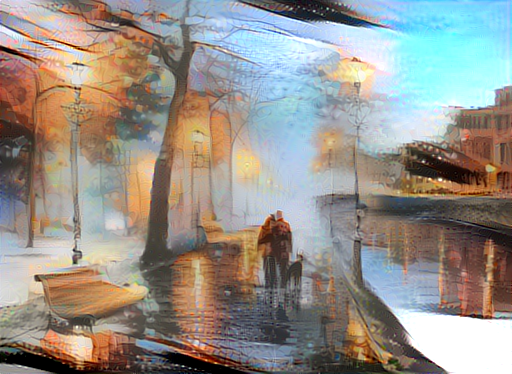
\includegraphics[width=0.8\linewidth]{brooklyn_night/out.png}
\end{center}
   \caption{The generated image after 1000 iterations, when using the photograph as the style image and the painting as the content image.}
\label{fig:long}
\label{fig:onecol}
\end{figure}

%------------------------------------------------------------------------
\section{Conclusion}

We reimplemented the algorithm for neural image transfer [1] to generate images that combined the content of a photograph and the style of an artwork and also a simple method of post-processing the generated images [8] to preserve the colors of the content image while maintaining the texture of the style image. This seems to work decently, producing good results after at least 500 iterations. 

There are many next steps that can be taken from this point. One example could be to try implementing the approaches to color mapping as discussed in [2] to achieve better results. Further steps could also be taken in respect to the work discussed under the Related Work section, such as optimizing the runtime of the neural net algorithm, extending image style transfers to video style transfers, and approaches to image style transfer that do not use neural nets.

%------------------------------------------------------------------------
\section{Individual Contribution}

vlee: I collaborated with the other team member to understand the algorithm for neural image transfer, make high-level decisions concerning the algorithm implementation process, set parameter values, and analyze the results. I took more responsibility for the implementation of preprocessing images, content loss, and postprocessing images for color mapping.

ssong: I collaborated with the other team member to understand the algorithm for neural image transfer, make high-level decisions concerning the algorithm implementation process, set parameter values, and analyze the results. I took more responsibility for the implementation of style representation (Gram matrices), and style loss.

%------------------------------------------------------------------------
\section{References}

[1] Leon A. Gatys, Alexander S. Ecker, and Matthias Bethge. A Neural Algorithm of Artistic Style. In: CoRR abs/1508.06576 (2015). url: http://arxiv.org/abs/1508.06576.

[2] Leon A. Gatys et al. Preserving Color in Neural Artistic Style Transfer. In: CoRR abs/1606.05897 (2016). url: http://arxiv.org/abs/1606.05897.

[3] Ulyanov, Dmitry, Vadim Lebedev, Andrea Vedaldi, and Victor Lempitsky. Texture Networks: Feed-forward Synthesis of Textures and Stylized Images (2016).

[4] Johnson, Justin, Alexandre Alahi, and Li Fei-Fei. Perceptual Losses for Real-Time Style Transfer and Super-Resolution (2016).

[5] Manuel Ruder, Alexey Dosovitskiy, Thomas Brox. Artistic Style Transfer for Videos (2016). url: https://arxiv.org/abs/1604.08610

[6] K. Simonyan and A. Zisserman. Very Deep Convolutional Networks for Large-Scale Image Recognition. arXiv:1409.1556 [cs], Sept. 2014. arXiv: 1409.1556.

[7] Y. Jia, E. Shelhamer, J. Donahue, S. Karayev, J. Long, R. Girshick, S. Guadarrama, and T. Darrell. Caffe: Convolutional
architecture for fast feature embedding. In Proceedings of the ACM International Conference on Multimedia, pages 675-678. ACM, 2014.

[8] https://github.com/jcjohnson/neural-style

% https://afremov.com/image.php?type=P&id=19095
[9] https://afremov.com/image.php?type=P\&id=19095

% http://images.mentalfloss.com/sites/default/files/styles/insert_main_wide_image/public/iStock_000026542107_Small.jpg
[10] http://images.mentalfloss.com/sites/default/files/styles/
insert\_main\_wide\_image/public/iStock\_000026542107\_Small.jpg

{\small
\bibliographystyle{ieee}
\bibliography{finalbib}
}

\end{document}
